\chapter{整体架构与技术选型}

\section{整体架构}
项目整体结构如图 \ref{server} 所示,共分为神经信息数据库,用户信息数据库以及网络服务器三部分组成。
\begin{figure}
\centering
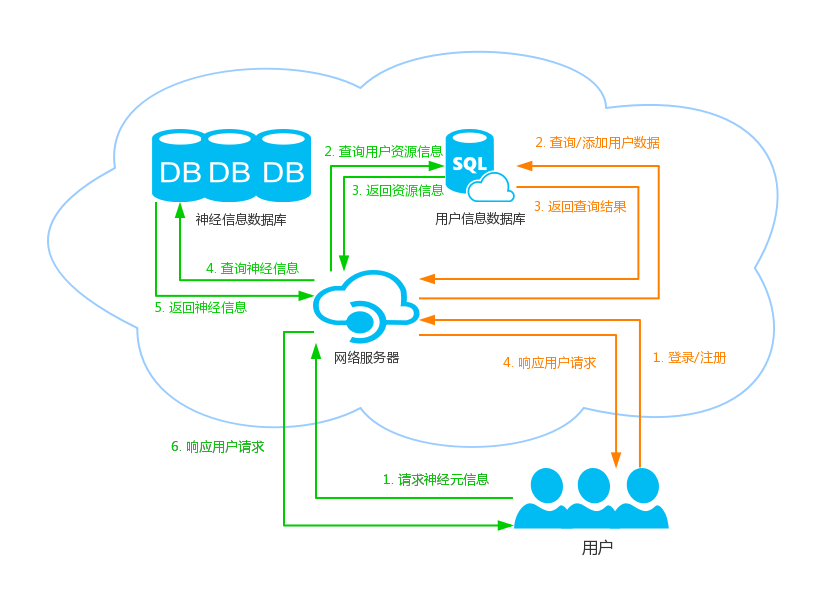
\includegraphics[width=148mm]{images/server}
\caption{项目整体架构}
\label{server}
\end{figure}
图中主要包含了两个方向的数据流,一个是用户信息数据流,另外一个是神经信息数据流。

\subsection{用户信息数据流}
用户信息数据流主要负责三件事情,一是验证用户身份,二是获取用户资源列表,三是检查用户行为是否有足够的权限。用户信息数据流可以抽象成如下几步:

1. 用户向网络服务器发送请求,登录平台或注册新用户

2. 网络服务器向用户信息数据库验证用户身份或添加新的用户信息

3. 用户信息数据库返回验证结果给网络服务器

4. 网络服务器将结果反馈给用户

\subsection{神经信息数据流}
神经信息数据流负责维护三对关系,用户和原始神经图片信息的关系,用户和数字重建结果直接的关系以及数字重建结果和原始图片信息之间的关系。神经信息数据流可以抽象成如下几步:

1. 用户像网络服务器请求神经元信息

2. 网络服务器利用用户信息数据流中保存的用户信息返回对应用户资源列表

3. 用户信息数据库返回用户资源列表给网络服务器

4. 网络服务器根据用户资源列表向神经信息数据库查询对应神经信息

5. 神经信息数据库返回对应神经信息给网络服务器

6. 网络服务器返回用户所需的神经信息用于前端的可视化展示

\section{技术选型}

\subsection{神经信息数据库}
神经信息数据库包含两部分数据,一部分是原始大脑切片显微镜图像,另外一部分是初步完成数字重建的 SWC 文件。使用 DVID 作为数据库,储存这些信息。DVID 是一个分布式面向图像的数据服务,主要用于图像分析与可视化。DVID 有如下特点:

1. 便于扩展数据类型,允许用户根据数据特点加速访问速度,减少储存空间,提供方便的 API。这为储存数字重建结果提供了便利。

2. 为分布式数据储存提供了类似于 GIT 的版本控制系统,在此基础之上我们可以解决多用户同时编辑产生冲突的问题。

3. 方便连接其他 API 如 Google BrainMaps 和 OpenConnectome 等。

4. 支持多分辨率图像数据,使得用户可以在不同尺度下观察图像信息。

在 DVID 的基础上,构建出原始大脑切片显微镜图像与数字重建结果的储存仓库,将数据储存抽象成数据存储服务,使得可以专注于完成核心算法和逻辑。

\subsection{用户信息数据库}
用户信息数据库包含多用户管理以及用户资源管理。使用 PostgreSQL 数据库储存这部分信息。PostgreSQL 最初由加州大学伯克利分校计算机系开发完成。在支持大部分 SQL 标准之上,提供了许多诸如复杂查询,多版本并行控制,事物完整性等现代特性\upcite{stonebraker1991postgres}。由于 PostreSQL 对标准 SQL 支持度较高,可以方便的和 DVID 联系起来,将用户信息和原始图像信息,数字重建结果对应起来。利用 PostgreSQL 支持的储存过程,事物以及多版本并行控制特性,我们可以方便的实现分布式,多用户实时编辑平台,并解决多用户同时编辑可能产生冲突的问题。

\subsection{网络服务器}
采用 Node.js 和 Express 完成网络应用开发。Node.js 是一个基于 Chrome V8 引起的 JavaScript 的运行环境。Node.js 使用了一个事件驱动、非阻塞式 I/O 的模型,使其轻量又高效\upcite{tilkov2010node}。Express 是一个基于 Node.js 平台的极简、灵活的 web 应用开发框架,提供丰富的 HTTP 快捷方式和任意排列组合的 Connect 中间件,帮助快速、简单的创建健壮、友好的 API。